\documentclass[english]{../thermomemo/thermomemo}
\pdfminorversion=4
\usepackage[utf8]{inputenc}

\usepackage{amsmath}
%\input{mathdef}
\usepackage[per-mode=symbol]{siunitx}
\usepackage[numbers]{natbib}
\usepackage{amsmath}
\usepackage{amssymb}
\usepackage{array}% improves tabular environment.
\usepackage{dcolumn}% also improves tabular environment, with decimal centring.

\usepackage{booktabs}
\usepackage{a4wide}
\usepackage{xspace}
\usepackage{todonotes}
\presetkeys{todonotes}{inline}{}
\usepackage{subcaption,caption}
\usepackage{tikz}
\usetikzlibrary{arrows}
\usetikzlibrary{snakes}
\usepackage{verbatim}
\usepackage{hyperref}
\hypersetup{
  colorlinks=true,
  linkcolor=blue,
  urlcolor=blue,
  citecolor=blue
}
%
% Egendefinerte
%
% Kolonnetyper for array.sty:
\newcolumntype{C}{>{$}c<{$}}% for å slippe å taste inn disse $
\newcolumntype{L}{>{$}l<{$}}% for å slippe å taste inn disse $
%
\newcommand*{\unit}[1]{\ensuremath{\,\mathrm{#1}}}
\newcommand*{\uunit}[1]{\ensuremath{\mathrm{#1}}}
%\newcommand*{\od}[3][]{\frac{\mathrm{d}^{#1}#2}{\mathrm{d}{#3}^{#1}}}% ordinary derivative
\newcommand*{\od}[3][]{\frac{\dif^{#1}#2}{\dif{#3}^{#1}}}% ordinary derivative
\newcommand*{\pd}[3][]{\frac{\partial^{#1}#2}{\partial{#3}^{#1}}}% partial derivative
\newcommand*{\pdc}[3]{\frac{\partial^{2}#1}{\partial{#2}\partial{#3}}}% partial derivative
\newcommand*{\pdt}[3][]{{\partial^{#1}#2}/{\partial{#3}^{#1}}}% partial
                                % derivative for inline use.
\newcommand{\pone}[3]{\frac{\partial #1}{\partial #2}_{#3}}% partial
                                % derivative with information of
                                % constant variables
\newcommand{\ponel}[3]{\frac{\partial #1}{\partial #2}\bigg|_{#3}} % partial derivative with information of constant variable. A line is added.
\newcommand{\ptwo}[3]{\frac{\partial^{2} #1}{\partial #2 \partial
    #3}} % partial differential in two different variables
\newcommand{\pdn}[3]{\frac{\partial^{#1}#2}{\partial{#3}^{#1}}}% partial derivative

% Total derivative:
\newcommand*{\ttd}[2]{\frac{\mathrm{D} #1}{\mathrm{D} #2}}
\newcommand*{\td}[2]{\frac{\mathrm{d} #1}{\mathrm{d} #2}}
\newcommand*{\ddt}{\frac{\partial}{\partial t}}
\newcommand*{\ddx}{\frac{\partial}{\partial x}}
% Vectors etc:
% For Computer Modern:

\DeclareMathAlphabet{\mathsfsl}{OT1}{cmss}{m}{sl}
\renewcommand*{\vec}[1]{\boldsymbol{#1}}%
\newcommand*{\vektor}[1]{\boldsymbol{#1}}%
\newcommand*{\tensor}[1]{\mathsfsl{#1}}% 2. order tensor
\newcommand*{\matr}[1]{\tensor{#1}}% matrix
\renewcommand*{\div}{\boldsymbol{\nabla\cdot}}% divergence
\newcommand*{\grad}{\boldsymbol{\nabla}}% gradient
% fancy differential from Claudio Beccari, TUGboat:
% adjusts spacing automatically
\makeatletter
\newcommand*{\dif}{\@ifnextchar^{\DIfF}{\DIfF^{}}}
\def\DIfF^#1{\mathop{\mathrm{\mathstrut d}}\nolimits^{#1}\gobblesp@ce}
\def\gobblesp@ce{\futurelet\diffarg\opsp@ce}
\def\opsp@ce{%
  \let\DiffSpace\!%
  \ifx\diffarg(%
    \let\DiffSpace\relax
  \else
    \ifx\diffarg[%
      \let\DiffSpace\relax
    \else
      \ifx\diffarg\{%
        \let\DiffSpace\relax
      \fi\fi\fi\DiffSpace}
\makeatother
%
\newcommand*{\me}{\mathrm{e}}% e is not a variable (2.718281828...)
%\newcommand*{\mi}{\mathrm{i}}%  nor i (\sqrt{-1})
\newcommand*{\mpi}{\uppi}% nor pi (3.141592...) (works for for Lucida)
%
% lav tekst-indeks/subscript/pedex
\newcommand*{\ped}[1]{\ensuremath{_{\text{#1}}}}
% høy tekst-indeks/superscript/apex
\newcommand*{\ap}[1]{\ensuremath{^{\text{#1}}}}
\newcommand*{\apr}[1]{\ensuremath{^{\mathrm{#1}}}}
\newcommand*{\pedr}[1]{\ensuremath{_{\mathrm{#1}}}}
%
\newcommand*{\volfrac}{\alpha}% volume fraction
\newcommand*{\surften}{\sigma}% coeff. of surface tension
\newcommand*{\curv}{\kappa}% curvature
\newcommand*{\ls}{\phi}% level-set function
\newcommand*{\ep}{\Phi}% electric potential
\newcommand*{\perm}{\varepsilon}% electric permittivity
\newcommand*{\visc}{\mu}% molecular (dymamic) viscosity
\newcommand*{\kvisc}{\nu}% kinematic viscosity
\newcommand*{\cfl}{C}% CFL number

\newcommand*{\cons}{\vec U}
\newcommand*{\flux}{\vec F}
\newcommand*{\dens}{\rho}
\newcommand*{\svol}{\ensuremath v}
\newcommand*{\temp}{\ensuremath T}
\newcommand*{\vel}{\ensuremath u}
\newcommand*{\mom}{\dens\vel}
\newcommand*{\toten}{\ensuremath E}
\newcommand*{\inten}{\ensuremath e}
\newcommand*{\press}{\ensuremath p}
\renewcommand*{\ss}{\ensuremath a}
\newcommand*{\jac}{\matr A}
%
\newcommand*{\abs}[1]{\lvert#1\rvert}
\newcommand*{\bigabs}[1]{\bigl\lvert#1\bigr\rvert}
\newcommand*{\biggabs}[1]{\biggl\lvert#1\biggr\rvert}
\newcommand*{\norm}[1]{\lVert#1\rVert}
%
\newcommand*{\e}[1]{\times 10^{#1}}
\newcommand*{\ex}[1]{\times 10^{#1}}%shorthand -- for use e.g. in tables
\newcommand*{\exi}[1]{10^{#1}}%shorthand -- for use e.g. in tables
\newcommand*{\nondim}[1]{\ensuremath{\mathit{#1}}}% italic iflg. ISO. (???)
\newcommand*{\rey}{\nondim{Re}}
\newcommand*{\acro}[1]{\textsc{\MakeLowercase{#1}}}%acronyms etc.

\newcommand{\nto}{\ensuremath{\mbox{N}_{\mbox{\scriptsize 2}}}}
\newcommand{\chfire}{\ensuremath{\mbox{CH}_{\mbox{\scriptsize 4}}}}
%\newcommand*{\checked}{\ding{51}}
\newcommand{\coto}{\ensuremath{\text{CO}_{\text{\scriptsize 2}}}}
\newcommand{\celsius}{\ensuremath{^\circ\text{C}}}
\newcommand{\clap}{Clapeyron~}
\newcommand{\subl}{\ensuremath{\text{sub}}}
\newcommand{\spec}{\text{spec}}
\newcommand{\sat}{\text{sat}}
\newcommand{\sol}{\text{sol}}
\newcommand{\liq}{\text{liq}}
\newcommand{\vap}{\text{vap}}
\newcommand{\amb}{\text{amb}}
\newcommand{\tr}{\text{tr}}
\newcommand{\crit}{\text{crit}}
\newcommand{\entr}{\ensuremath{\text{s}}}
\newcommand{\fus}{\text{fus}}
\newcommand{\flash}[1]{\ensuremath{#1\text{-flash}}}
\newcommand{\spce}[2]{\ensuremath{#1\, #2\text{ space}}}
\newcommand{\spanwagner}{\text{Span--Wagner}}
\newcommand{\triplepoint}{\text{TP triple point}}
\newcommand{\wrpt}{\text{with respect to~}}
\newcommand{\tpd}{\ensuremath{\text{tpd}}\xspace}
\newcommand{\TPD}{\ensuremath{\text{TPD}}\xspace}

\title{Stability and critical points of mixtures}
\author{Morten Hammer}

\graphicspath{{gfx/}}

\begin{document}
\frontmatter
\tableofcontents
\section{Introduction}
This memo is to present methods for calculating stability and critical points of
mixture. Background information on stability of mixtures and the calculation of
critical points is found in \citet{Reid1977}, \citet{Heidemann1980},
\citet{Michelsen1984} and \citet[Chap. 9]{Michelsen2007}.
\section{Limit of stability formulated in temperature and pressure}
\label{sec:tp_fomulation}
The stability criterion for a mixture with composition $z$, formulated
in temperature and pressure, is given by
\begin{equation}
  \label{eq:TPDorg}
  \TPD(\vektor{w}) = \underset{i}{\sum}w_i\left(\mu_i(\vektor{w})-\mu_i(\vektor{z})\right),
\end{equation}
where \TPD is the tangent plane distance function, and $\mu$ is the
chemical potential. If looking at global stability, $\vektor{w}$ is any
composition. In the case of local stability, $\vektor{w}$ is any perturbation
of $\vektor{z}$. If \TPD is non-negative the mixture $\vektor{z}$ is stable.

A modified stability condition for a reduced tangent plane
distance \tpd, is given in Equation \ref{eq:tpd}. \tpd is evaluated
using composition variables treated as mole numbers, $\vektor{Y}$, instead of
composition, and have better properties and are easier to solve
numerically that the $TPD$ formulation.
\begin{equation}
  \tpd(\vektor{Y}) = 1.0 + \underset{i}{\sum}Y_i\left(\ln Y_i + \ln \varphi_i(\vektor{Y})-\ln z_i - \ln \varphi_i(\vektor{z})\right).
  \label{eq:tpd}
\end{equation}
Here $\varphi$ is the fugacity.

Differentiating Equation \ref{eq:tpd}, we get
\begin{align}
  \vektor{g} &= \pd{\tpd}{\vektor{Y}} = \ln Y_i + \ln \varphi_i(\vektor{Y})-\ln z_i - \ln \varphi_i(\vektor{z}),\\
  H_{ij} &= \frac{\partial^2\tpd}{\partial Y_i \partial Y_j} = \frac{\delta_{ij}}{Y_i} + \frac{\partial \ln \varphi_i(\vektor{Y})}{Y_j}.
  \label{eq:dtpd}
\end{align}

Looking at local stability of a mixture phase with composition $\vektor{z}$, a
perturbation of $\vektor{z}$, $\vektor{Y} = \vektor{z} + \vektor{e}$, for small $\vektor{e}$ must give a positive
\tpd. A Taylor series expansion from $\vektor{Y}=\vektor{z}$ yields,
\begin{align}
  \tpd(\vektor{Y}) =& \tpd(\vektor{z}) + \left(\pd{\tpd}{\vektor{z}}\right)^\intercal\vektor{e} + \frac{1}{2}\vektor{e}^\intercal\left(\pd[2]{\tpd}{\vektor{z}}\right)\vektor{e} + \dots \\
  =& \tpd + \vektor{g}^\intercal \vektor{e} + \frac{1}{2}\vektor{e}^\intercal\vektor{H}\vektor{e} + \dots.
  \label{eq:tpdTaylor}
\end{align}
Since $\tpd(\vektor{z}) = 0$ and $\vektor{g}(\vektor{z}) = 0$, the local stability limit therefore become,
\begin{equation}
  \text{det}\left(H\right) = 0,
  \label{eq:detM}
\end{equation}
or equivalent $\lambda_{\text{min}} = 0$, where $\lambda_{\text{min}}$
is the minimum eigenvalue of $\vektor{H}$.

To improve the scaling and the numerical properties of the problem,
\citet{Michelsen1984} introduces a scaling of the composition
variables,
\begin{equation}
  \label{eq:X}
  X_i = \frac{Y_i-z_i}{\sqrt{z_i}}.
\end{equation}
Further $X_i = s u_i$, where $\vektor{u}$ is a normalized vector,
$\vektor{u}^\intercal\vektor{u} = 1$. The perturbed composition then becomes,
\begin{equation}
  \label{eq:Y}
  Y_i = z_i + s u_i\sqrt{z_i}.
\end{equation}
Differentiating Equation \ref{eq:tpd} \wrpt $X_i$ we get,
\begin{align}
  \pd{\tpd}{X_i} = \sqrt{z_i}g_i,\\
  \frac{\partial^2\tpd}{\partial X_i \partial X_j} = B_{ij} &=  \sqrt{z_i}\sqrt{z_j}H_{ij}.
  \label{eq:dtpdX}
\end{align}

Further, if we let $\vektor{u}$ be the eigenvector corresponding to the smallest
eigenvalue, $\lambda_{\text{min}}$, of $\vektor{B}$, we have
\begin{equation}
  \label{eq:b}
  b = \frac{1}{2}\vektor{u}^{\top}\vektor{B}\vektor{u} = \frac{1}{2} \lambda_{\text{min}}.
\end{equation}

\subsection{Numerical solver}
Solving for $b = 0$ in Equation \ref{eq:b}, for a specified pressure
or temperature is complicated. The solution value ($T$ ot $p$) will
lie near the value ($T$ ot $p$) where the underlying equation of state
loses a density root (phase). A discontinuity will therefore be
located close to the solution, excluding the possibility of using a
bracketing solver, unless the position where the phase root disappears
is know. If we are dealing with a cubic equation of state, the
position where the model looses a density root can easily be
determine, otherwise not. See Figure \ref{fig:meta_init}.
\begin{figure}[h]
  \centering
  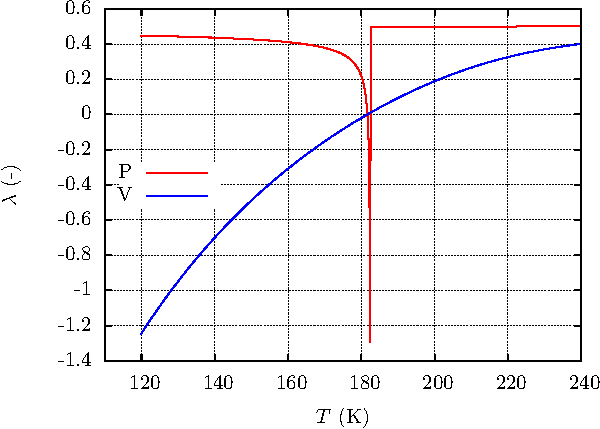
\includegraphics[width=0.6\textwidth]{meta_init}
  \caption{Minimum eigenvalue plotted as a function of $T$ for given
    pressure, $P$ and for given specific volume, $V$. The
    meta-stable limit is located at $T=\SI{181.65}{\kelvin}$. The $TP$
    line have a discontinuity (phase disappear) located close to the
    meta-stable limit, while the $TV$ line is monotonous. The plot is
    generated for a mixture of \SI{90}{\percent} methane and
    \SI{10}{\percent} ethane.}
  \label{fig:meta_init}
\end{figure}

Specifying a pressure and solving for a temperature at the meta-stable
limit, has been found possible for low pressures. The saturation
temperature, when treating the fluid as a pure fluid, at low
pressures, can be used as initial value of the search for a
meta-stable limit of a gas/liquid. We then know that the solution will
lie below (gas) and above (liquid) the initial guess. Using a
Newton-Raphson (NR) solver we will take steps in a direction towards
the solution, but with the possibility of overshooting the
solution. Since the eigenvalue of the stability matrix, $\vektor{B}$,
changes abruptly when a phase disappears, and another phase is selected
by the EOS density solver, a line search is used to back track if the
search step becomes to large.

The NR solver must use numerical differentials since analytical
differentials are difficult to derive in the general case.

For larger pressures, where the metastable limits of the gas and the
liquid come close together, it has proven difficult to guaranty
solution to the correct meta-stable limit. To overcome this problem,
an alternative formulation is needed.

\section{Alternative formulation}
Michelsen and Heidemann \cite{Heidemann1980} suggest that a
formulation in the variables $T$ and $v$ is more robust than the $P$
and $T$ formulation. One reason for this is that following the meta
stable limit, the volume will be monotonous.

The Heidemann tangent plane distance for $T$ and $v$ are given as,
\begin{equation}
  \label{eq:tpd_TV}
  \TPD\left(T,V,\mathbf{Y}\right) =
 A\left(T,V,\mathbf{Y}\right) - A\left(T,V_0,\mathbf{z}\right) +
 P\left(T,V_0,\mathbf{z}\right)\left(V - V_0\right) -
 \underset{j}{\sum}\mu\left(T,V_0,\mathbf{z}\right)\left(Y_j - z_j\right)
 .
\end{equation}

The Michelsen \citet[Chap. 9]{Michelsen2007} reduced tangent plane distance for $T$ and $v$ are given as,
\begin{equation}
  \label{eq:tpd_TV_M}
  \tpd(T,V,\mathbf{Y}) =
  \underset{j}{\sum}Y_j\left[\ln f_j \left(T,V,\mathbf{Y}\right) -
    \ln f_j\left(T,V_0,\mathbf{z}\right)\right] -
  \left[P\left(T,V,\mathbf{Y}\right) - P_0\right]\frac{V}{RT}
  .
\end{equation}

The Helmholtz energy can be written as follows,
\begin{equation}
  \label{eq:A}
 A\left(T,V,\mathbf{Y}\right) = - P\left(T,V,\mathbf{Y}\right)V +
 \underset{j}{\sum}Y_j\mu\left(T,V,\mathbf{Y}\right)
 .
\end{equation}

The fugacity coefficient definition
\begin{equation}
  \label{eq:fugacity}
  R T \ln f_j\left(T,V,\mathbf{Y}\right) =
  \pd{A\left(T,V,\mathbf{Y}\right)}{Y_j} = \mu_j \left(T,V,\mathbf{Y}\right).
\end{equation}
give the following relation:
\begin{equation}
  \label{eq:A2}
 A\left(T,V,\mathbf{Y}\right) = - P\left(T,V,\mathbf{Y}\right)V +
 \underset{j}{\sum}Y_j\ln f_j\left(T,V,\mathbf{Y}\right).
\end{equation}

Note that we are not working with the reduced Helmholtz energy, but
the real Helmholtz energy.

Using Equations \ref{eq:A}, \ref{eq:fugacity} and \ref{eq:A2}, and
$V=V_0$ it is seen that Equation \ref{eq:tpd_TV} and Equation
\ref{eq:tpd_TV_M} represent the same stability criteria:
\begin{align}
  \label{eq:tpd_TV_M2}
  tpd(T,V,\mathbf{Y}) =&
  \underset{j}{\sum}Y_j\left[\ln f_j \left(T,V,\mathbf{Y}\right) -
    \ln f_j\left(T,V_0,\mathbf{z}\right)\right] -
  \left[P\left(T,V,\mathbf{Y}\right) - P_0\right]\frac{V}{RT},\\
  =& \frac{1}{RT}\left(-P\left(T,V,\mathbf{Y}\right) V +
     \underset{j}{\sum}Y_j\mu_j \left(T,V,\mathbf{Y}\right) \right)\\
  & - \frac{1}{RT}\left( - P_0V_0 + P_0\left(V_0-V\right)
    -\underset{j}{\sum}\left(Y_j - z_j + z_j\right)\mu_j\left(T,V_0,\mathbf{z}\right)
  \right)
  ,\\
  =& \frac{1}{RT}\left( A\left(T,V,\mathbf{Y}\right) -
     A\left(T,V_0,\mathbf{z}\right) + P_0\left(V_0-V\right) - \underset{j}{\sum}\left(Y_j - z_j\right)\mu_j\left(T,V_0,\mathbf{z}\right)\right),
\end{align}

Differentiating Equation \ref{eq:tpd_TV_M} w.r.t. $n_i$, and using $V=V_0$ we
get
\begin{equation}
  \label{eq:tpd_TV_n}
  g_i =
 \ln f_i\left(T,V_0,\mathbf{Y}\right) +
 \ln f_i\left(T,V_0,\mathbf{z}\right),
\end{equation}
and
\begin{equation}
  \label{eq:tpd_TV_h}
  h_{ij} =
 \ln f_{ij}\left(T,V,\mathbf{Y}\right) .
\end{equation}

The same variable scaling is used for this formulation, as in the
previous section (Equation \ref{eq:X}). Using the temperature-pressure
formulation to calculate an initial point, Section
\ref{sec:tp_fomulation}, for a low pressure, the entire meta-stable
limit can be mapped using steps in the volume variable. Stepping with
fixed increments in $\ln v$ was found optimal considering resolution of
the line.

An example, plotting the meta-stable limit together with the phase
envelope for a mixture of \SI{90}{\percent} methane and
\SI{10}{\percent} ethane, is plotted in Figure \ref{fig:meta}.
\begin{figure}[h]
  \centering
  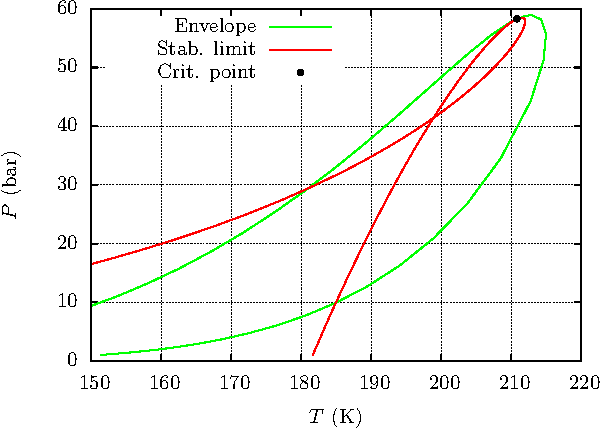
\includegraphics[width=0.6\textwidth]{meta}
  \caption{Phase envelope and meta-stable limit plotted for a mixture
    of \SI{90}{\percent} methane and \SI{10}{\percent} ethane. The
    critical point is plotted using a black dot.}
  \label{fig:meta}
\end{figure}


\subsection{Single component}
The pure fluid stability limit is the well-known,
\begin{equation}
  \label{eq:dpdv_t}
  \left(\pd{p}{v}\right)_T = 0.
\end{equation}

The mapping of the meta-stable limit for pure fluids currently use a
solver for Equation \ref{eq:dpdv_t}. For robust and fast mapping,
extrapolation of volume is performed between each step in temperature.

%\todo{Investigate if multi-component approach can be used for single components as well.}

An example, plotting the meta-stable limit together with the
saturation line for pure \coto, is plotted in Figure
\ref{fig:singleMeta}.
\begin{figure}[h]
  \centering
  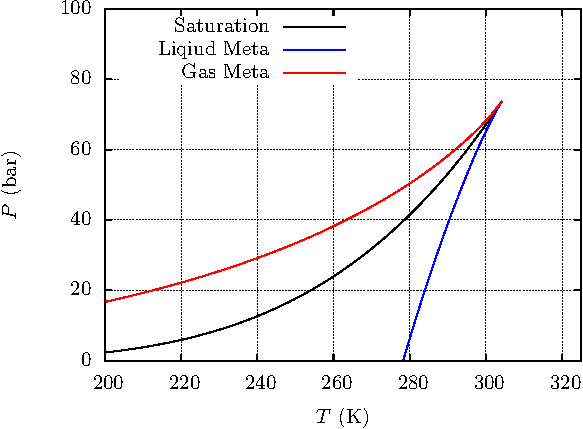
\includegraphics[width=0.6\textwidth]{singleMeta}
  \caption{Saturation line and meta-stable limit plotted for pure
    \coto. Peng-Robinson equation of state with van der Waals mixing
    rules are applied.}
  \label{fig:singleMeta}
\end{figure}

\section{Critical point}
``A critical point is a stable point which lies on the stability
limit.'' - \citet{Heidemann1980}. The implications from this is that,
if \tpd is Taylor expanded, the cubic form must vanish. See
\cite{Heidemann1980} for more details.

% The critical will lie on the meta-stable line and also satisfying,
% \begin{equation}
%   q_{ijk} = \left(\frac{\partial^3\tpd}{\partial z_i \partial z_j \partial z_k}\right)_{T,V\text{ or }P} % \Delta z_i \Delta z_j \Delta z_k.
%   \label{eq:q}
% \end{equation}

\subsection{Critical point solver}
Since the third order differentials of \tpd typically is difficult and
time consuming to construct analytically, \citet{Michelsen1984}
developed an approach to solve for a critical point numerically
without calculating these differentials. The main components of this
algorithm is given below for the formulation in temperature an volume.
Using $F = \tpd$, and Taylor expanding in $s$, we get
\begin{align}
F(\mathbf{X} = s\mathbf{u}) = F_1(s) = \overset{\infty}{\underset{m=0}{\sum}}\left(\frac{s^m}{m!}\right)\left(\frac{\partial^m F_1}{\partial s^m}\right)_{s=0} = as + bs^2 + cs^3 + ds^4 + \mathcal{O}(s^5),
\label{eq:sTaylor}
\end{align}
since $F_1(s=0) = 0$. Further,
$a = \left(\partial F_1/\partial s\right)_{s=0} =
\underset{i}{\sum}\sqrt{z_i}u_ig_i(s=0)=0$. For $b$ we have,
\begin{equation}
b = \frac{1}{2}{\underset{i,j}{\sum}}B_{ij}u_iu_j = \frac{1}{2}\mathbf{u}^\intercal \mathbf{B} \mathbf{u},
\label{eq:bdef}
\end{equation}
identical to the definition in Equation \ref{eq:b}. The smallest value
of $b$ is found by choosing $\mathbf{u}$ to be the eigenvector
corresponding to the minimum eigenvalue of $\mathbf{B}$. We then get,
\begin{equation}
\mathbf{B} \mathbf{u} = \lambda_{\text{min}} \mathbf{u}, \mathbf{u}^\intercal\mathbf{u} = 1
\label{eq:brelation}
\end{equation}

For $c$ we have,
\begin{equation}
  c = \frac{1}{6}{\underset{i,j,k}{\sum}}q_{ijk}u_iu_ju_k.
\label{eq:cdef}
\end{equation}

Differentiating Equation \ref{eq:sTaylor} \wrpt $s$, we get,
\begin{align}
\pd{F_1}{s} =  2bs + 3cs^2 + 4ds^3 + \mathcal{O}(s^4),
\label{eq:sTaylords}
\end{align}
and this equals
\begin{align}
\pd{F_1}{s} = \underset{i}{\sum}\pd{F}{Y_i}\pd{Y_i}{s} = \underset{i}{\sum}\sqrt{z_i}u_ig_i.
\label{eq:dfds}
\end{align}
Evaluating at $s=\epsilon$ and $s=-\epsilon$, we get
\begin{align}
\left(\pd{F_1}{s}\right)_{\epsilon} &= 2b\epsilon + 3c\epsilon^2 + 4d\epsilon^3 + \mathcal{O}(\epsilon^4),\\
\left(\pd{F_1}{s}\right)_{-\epsilon} &= -2b\epsilon + 3c\epsilon^2 - 4d\epsilon^3 + \mathcal{O}(\epsilon^4).\\
\label{eq:dfdseps}
\end{align}
Adding the Equations above we get a Equation for $c$,
\begin{align}
c = \frac{1}{6\epsilon^2}\left(\left(\pd{F_1}{s}\right)_{\epsilon} + \left(\pd{F_1}{s}\right)_{-\epsilon}\right) + \mathcal{O}(\epsilon^2).
\label{eq:c}
\end{align}
\subsubsection{Critical point solver Jacobean}
In order to construct a Newton-Raphson solver differentials for the Jaocobian is
required.  Differentiating Equation \ref{eq:brelation} \wrpt temperature, we get
the relation,
\begin{equation}
\mathbf{B}_T \mathbf{u} + \mathbf{B} \mathbf{u}_T = \lambda_{T} \mathbf{u} + \lambda_{\text{min}} \mathbf{u}_T, \mathbf{u}^\intercal\mathbf{u}_T = 0
\label{eq:breldiffT}
\end{equation}
Multiplying with $\mathbf{u}^\intercal$, and simplifying we get,
\begin{align}
\mathbf{u}^\intercal \mathbf{B}_T \mathbf{u} + \mathbf{u}^\intercal\mathbf{B} \mathbf{u}_T &= \lambda_{T} \mathbf{u}^\intercal\mathbf{u} + \lambda_{\text{min}} \mathbf{u}^\intercal\mathbf{u}_T,\\
\mathbf{u}^\intercal \mathbf{B}_T \mathbf{u}  &= \lambda_{T}.
\label{eq:breldiffTuT}
\end{align}
Rearranging Equation \ref{eq:breldiffT}, we get
\begin{equation}
\left(\mathbf{B} - \lambda_{\text{min}}I\right) \mathbf{u}_T = \lambda_{T} \mathbf{u}  - \mathbf{B}_T \mathbf{u}.
\label{eq:breldiffTR}
\end{equation}
We see that if $\mathbf{B}_T \mathbf{u}$ is known, it is possible to
find $\mathbf{u}_T$. The elements of $\mathbf{B}_T \mathbf{u}$, is
\begin{align}
\label{eq:Btu}
  \left(\mathbf{B}_T \mathbf{u}\right)_i &= \sqrt{z_i}\underset{j}{\sum}\sqrt{z_j}u_j \pd{\ln f_{ij}}{T} = \sqrt{z_i} \pd{}{s}\left(\pd{\ln f_{i}}{T}\right)_{s=0} \\ 
                                         &\approx \sqrt{z_i} \left(\frac{1}{2\epsilon}\right)\left[\left(\pd{\ln f_{i}}{T}\right)_{s=\epsilon} - \left(\pd{\ln f_{i}}{T}\right)_{s=-\epsilon} \right].
\end{align}
Using $\mathbf{B}_T \mathbf{u}$, $\lambda_T$ is determined, and further $b_T = \lambda_T/2$. To determine $c_T$, Equation \ref{eq:sTaylor} is used,
\begin{align}
\pd{F_1}{T} = b_Ts^2 + c_Ts^3 + d_Ts^4 + \mathcal{O}(s^5).
\label{eq:dF1dT_Taylor}
\end{align}
Further differentiating Equation \ref{eq:tpd_TV_M}, we get
\begin{align}
\label{eq:dF1dT}
\pd{F_1}{T} &= \pd{\tpd}{T} +
  \underset{j}{\sum}\pd{\tpd}{Y_j}\pd{Y_j}{T},\\
\pd{\tpd}{T} &= \underset{j}{\sum}Y_j\left[\ln f_{jT} \left(\mathbf{Y}\right) -
     \ln f_{jT}\left(\mathbf{z}\right)\right] -
   \left[P_T\left(\mathbf{Y}\right) -
               P_T\left(\mathbf{z}\right)\right]\frac{V}{RT} \\ 
            &+\left[P\left(\mathbf{Y}\right) - P\left(\mathbf{z}\right)\right]\frac{V}{RT^2}\\
\pd{\tpd}{Y_j}\pd{Y_j}{T} &=g_j\sqrt{z_j}s(\mathbf{u}_T)_j
\end{align}
Evaluating equations \ref{eq:dF1dT} and \ref{eq:dF1dT_Taylor} at $\epsilon$ and $-\epsilon$ and combining, we get,
\begin{align}
c_T = \frac{1}{2\epsilon^3}\left(\left(\pd{F_1}{T}\right)_{\epsilon} - \left(\pd{F_1}{T}\right)_{-\epsilon}\right) + \mathcal{O}(\epsilon^2).
\label{eq:cT}
\end{align}
The differentials \wrpt volume can be determined in the same manner.

% \ref{eq:A}
% \begin{align}
%   \label{eq:dA}
%  \pd{A}{n_i} &= - P_iV + \mu_i
%  \underset{j}{\sum}n_j\pd{\mu}{n_i} = \mu_i \\ 
%  P_iV &= \underset{j}{\sum}n_j\pd{\mu}{n_i} \\
% F_1(T,V,n(T,V)) &=
%   \underset{j}{\sum}n_j\left[\ln f_j \left(T,V,\mathbf{n}\right) -
%     \ln f_j\left(T,V_0,\mathbf{z}\right)\right] -
%   \left[P\left(T,V,\mathbf{n}\right) - P_0\right]\frac{V}{RT}\\
%   \pd{F_1}{n_i} &= \ln f_i \left(T,V,\mathbf{n}\right) + \ln
%                   f_i\left(T,V_0,\mathbf{z}\right) + \underset{j}{\sum}n_j\left[\ln f_{ji} \left(T,V,\mathbf{n}\right) -
%     \ln f_{ji}\left(T,V_0,\mathbf{z}\right)\right] -
%    \left[P_i\left(T,V,\mathbf{n}\right) - P_{0,i}\right]\frac{V}{RT}\\
% \left[P\left(T,V,\mathbf{n}\right) - P_0\right]\frac{V}{RT}
% \end{align}
\clearpage
\bibliographystyle{plainnat}
\bibliography{../thermopack}

\end{document}
